\subsection{Scope}
The \app system is a dynamic web application fostering collaborative coding experiences for both students and educators. On this platform, students actively engage in tournaments and code kata battles to showcase their skills and monitor individual progress. 
Educators also play a crucial role in taking care of organizing tournaments and designing battles.

\app is integrated with GitHub, to leverage the GitHub abilities to store different versions of a coding project. For every battle generated on CodeKataBattle, a dedicated GitHub repository is created after the registration deadline of the battle expires. From that moment, students are able to push their code solutions for the battle in a personal repository that is forked by the one created as a reference by \app. 
Every student willing to participate in a battle, also has to autonomously develop a GitHub workflow (through GitHub Actions) in order to fire a notification from GitHub to \app every time a commit is performed on his/her repository.
When \app receives a notification from GitHub, it pulls the source code from the remote GitHub repository and automatically computes the score to assign to that solution based on some aspects like number of test cases passed, time went by from the beginning of the battle and static analysis on the source code run by an external static analysis tool.

Both tournaments and battles have rankings, that are kept updated anytime by \app until the battle or the tournament ends. When a battle ends, all students involved in the battle are notified, and the enclosing tournament ranking updated accordingly. When a tournament is closed by the educator who created it all students that took part in the tournament are notified. The final ranking of the tournament is also published and the badges are assigned to students who deserve them.

This document offers a finer insight on the design decisions that have been taken in order to implement the \app platform. From a very high-level standpoint, \app is first of all a web application. This choice is relevant because it allows a straightforward and easy access to the functionalities of the application from any client device equipped with an internet connection. 

The internal architecture follows the microservices architectural style, as all major functionalities of the system are scattered among different programs. The microservice architectural style promotes a more structured way of developing an application, by loosely coupling the different components and therefore boost maintainability and scalability. It also has a great impact on the development process when working with a team of developers, as each microservice can be designed independently from the others.
From a deployment point of view, the \app platform can be described as a three-tier architecture, since a single server runs all microservices, clients can connect to that server and the microservices can contact a remote database server for persistent data storage and manipulation. This structure of the system is shown more in detail in the following of the document. 
As for the data layer, the \app is built on a shared database, that all microservices can access. This way of thinking the data layer simplified data management, especially in situations where the data content managed by different microservices is often times related and logically interconnected.
Finally, some architectural patterns are employed in the design to allow an effective communication between microservices. \app microservices expose RESTful APIs to receive requests from the outside and respond with data (or to provide some sort of computation on data). An event-driven approach is also employed internally to improve performance and reduce coupling between microservices.
A Model-View-Controller pattern is also adopted in order to separate concerns between the software components that have to manage incoming requests and showing graphical user interfaces.

All these architectural choices are just mentioned here to provide an overview of the system, they will be better explained and unpacked down the line of this document.


\begin{minipage}{\linewidth}

The following image shows the major components of the \app system.

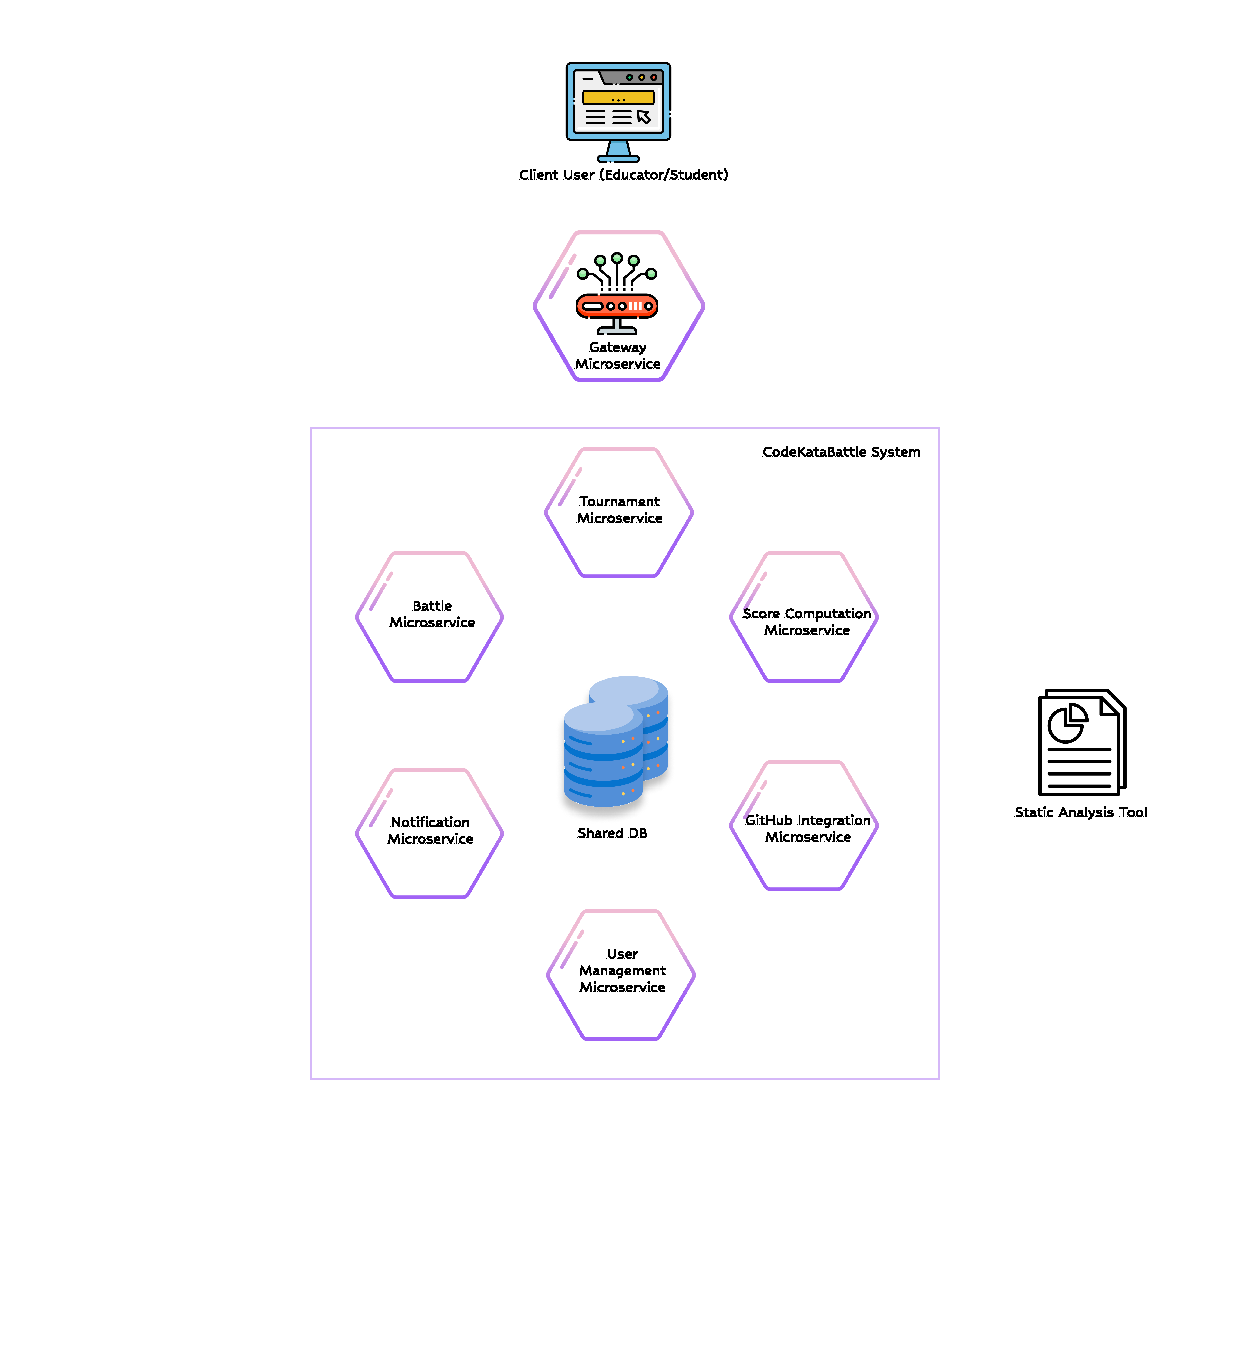
\includegraphics[width=\linewidth,page=1]{OverViewDiag}
\captionof{figure}{High-level view of the major components}

\end{minipage}
